\documentclass{article}
\usepackage{graphicx}
\usepackage[margin=1.5cm]{geometry}
\usepackage{amsmath}

\begin{document}

\title{Thursday Reading Assessment: Unit 8, Momentum}
\author{Prof. Jordan C. Hanson}

\maketitle

\section{Memory Bank}

\begin{itemize}
\item $\vec{p} = m\vec{v}$ ... Definition of momentum.
\item $\vec{p}_{\rm 1} + \vec{p}_{\rm 2} = \vec{p}_{\rm 1}~' + \vec{p}_{\rm 2}~'$ ... Momentum conservation for two objects interacting.
\end{itemize}

\section{Momentum}

\begin{enumerate}
\item
\begin{figure}[ht]
\centering
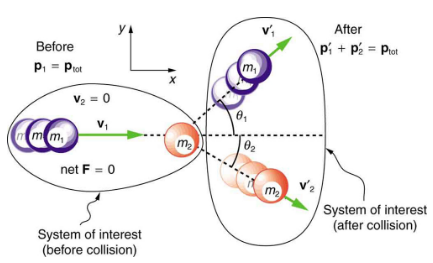
\includegraphics[width=0.4\textwidth]{collision2.png}
\caption{\label{fig:collision} A particle interacts with one at rest.}
\end{figure}
Suppose a mass $m_1$ approaches another mass $m_2$ with velocity $v_{\rm 1}$, while $m_2$ is at rest.  Break the momenta into x and y-components to show:
\begin{align}
m_1 v_{1} &= m_1 v_{1}'\cos\theta_1 + m_2 v_{2}'\cos\theta_2 \\
0 &= m_1 v_{1}'\sin\theta_1 + m_2 v_{2}'\sin\theta_2
\end{align}
Equation 1 applies to the x-coordinate, and Equation 2 applies to the y-coordinate.  \\ \vspace{2cm}
\item Let $m_1 = 0.1$ kg, and $m_2 = 0.1$ kg.  Also, $\theta_1$ is observed to be 30 degrees, and $\theta_2$ is observed to be 60 degrees.  If $v_{\rm 1}' = 1.0$ m/s, what is $v_{\rm 2}'$?
\end{enumerate}
\end{document}
